We can get the results of DL analysis in only less than 20 seconds after determining the target area and clicking the analyze button. The effort and hassle of using the DL was reduced to a minimum. However it also means we have to wait 20 seconds. It takes about 10 seconds to analyze 1920×1080 image for the computer with NVIDIA GeForce GTX 1080 Ti and a few seconds to transfer the result image files.

We were faced with the limitations of the Raspberry Pi's performance. Even just playing the video stream transfored from USB-connected microscopic camera, FPS drops. And there was also a delay to alpha composite the result image on the original one. The low performance of the hardware was detracting to the user experience of the client software.

\begin{figure}[t]\centering
  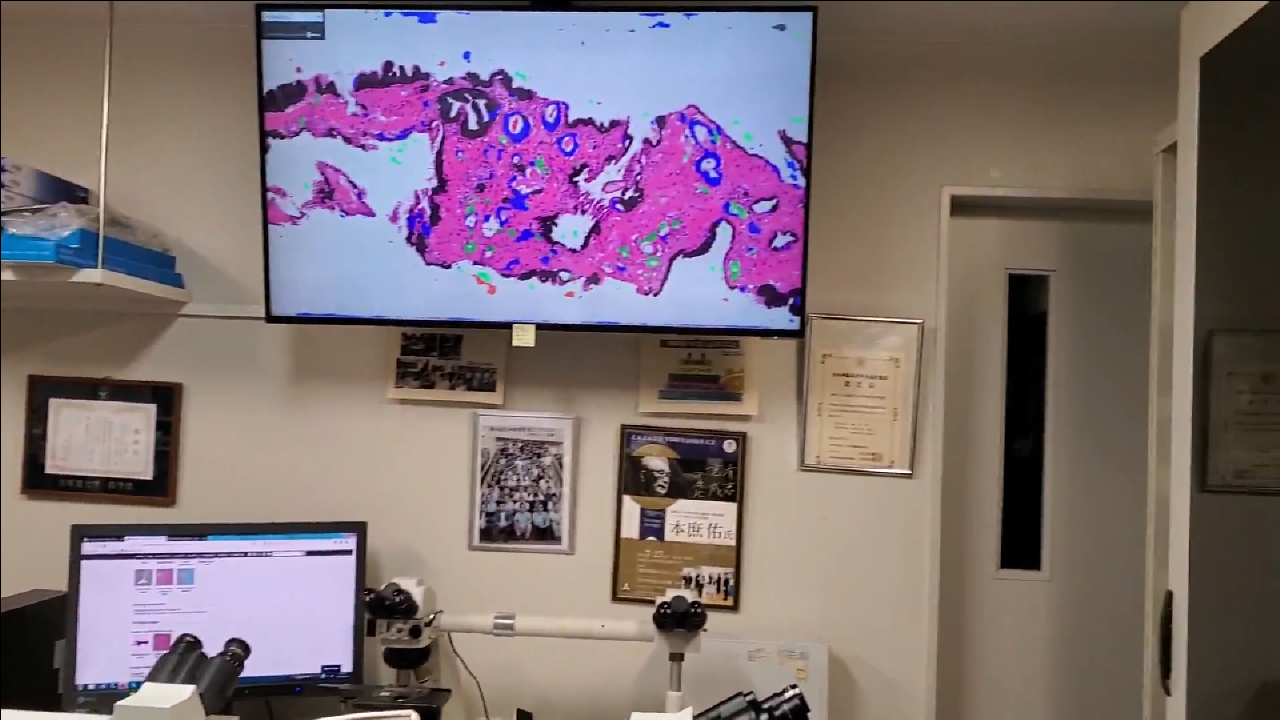
\includegraphics[keepaspectratio]{assets/thumb.png}
  \caption{The client application in action (\href{https://drive.google.com/file/d/16hUGZ2jU2Def9N5ozNaZnLvjnWc-kkNP/view}{Link to the movie})}
  \label{fig:in_action}
\end{figure}

We found they were grateful for the function just to save the image of the view microscopic view without any analytics. Up until now, microscopic camera was connected to display directyl via HDMI.  With the Raspberry Pi in between the camera and the display, we can now take photograph and analyze in addition to usage so far.  Users experienced as if the microscope camera was augmented in functional extension of itself.


